\documentclass[../../main.tex]{subfiles}

\begin{document}

Um herauszufinden, welchen Wert eine Unbekannte (also normalerweise $x$) haben muss, um eine Gleichung zu erfüllen, muss sie \emph{isoliert} werden: Die Gewichte und Gegenstände auf der Waage müssen so umsortiert werden, dass sich sofort das Gewicht des Gegenstandes ablesen lässt. Im folgenden Beispiel siehst du, dass du dann sofort ablesen kannst, welchen Wert die Unbekannte $x$ hat (bzw. wie viel die blaue Kugel wiegt).

\begin{example}{}
    \parpic[r]{
        \begin{linearEquation}
            %Füllung linke Waagschale
            \node[white,marble,inner sep=.12cm] at (-1,0.35) {$x$};
            %Füllung rechte Waagschale
            \fill (0.75,0.25) -- (1.25,0.25) -- (1.2,0.65) -- (0.8,0.65) -- cycle;
            \draw[line width=0.75mm] (1,0.71) circle[radius=0.06cm];
            \node[white] at (1,0.45) {$42$};
        \end{linearEquation}
    }
    
    In der linken Waagschale befindet sich hier nur die Kugel, deren Gewicht wir gern herausfinden würden. Die Kugel ist \emph{isoliert}. Auf der rechten Seite befindet sich nur ein einzelnes Gewicht.
    
    \picskip{5}
    Da wir nun wissen, dass die Waage sich gerade im Gleichgewicht befindet, muss die Kugel links natürlich genau so viel wiegen wie das Gewicht auf der rechten Seite. Sie muss also ein Gewicht von 42 haben.
    
    Nennen wir das Gewicht der Kugel wieder $x$, so stellt die Waage die Gleichung $x=42$ dar -- eine Gleichung, die uns sofort verrät, dass $x$ den Wert 42 haben muss.
\end{example}

Unser Ziel beim Lösen von Gleichungen ist es, die Gleichung in eine Form wie im letzten Beispiel zu bringen, in der sich die Lösung sofort ablesen lässt, also
\[x=\langle\text{Term ohne } x\rangle.\]
Die Variable $x$ steht allein auf der linken Seite und kommt auf der rechten Seite nicht vor. Den Prozess, eine Gleichung so umzuformen, dass das $x$ am Ende alleine steht, nennt man \textbf{\enquote{die Gleichung nach \emph{x} auflösen}} (oder allgemein, ohne den Namen der Unbekannten zu nennen: \emph{die Gleichung auflösen}). 

In diesem Kapitel lernst du, wie sich dies für \textbf{lineare Gleichungen} bewerkstelligen lässt. Lineare Gleichungen sind eine bestimmte Art von Gleichungen, die sich vergleichsweise einfach lösen lassen.

\begin{example}{}
    Die Gleichungen $x=19, x=5$ und $x=-7$ sind bereits nach $x$ aufgelöst, da das $x$ allein auf der linken Seite steht und auf der rechten Seite jeweils nicht vorkommt.
\end{example}
\begin{example}{}
    Die Gleichung $3x+15=(x-2)^2-7$ ist \emph{nicht} nach $x$ aufgelöst, denn das $x$ ist nicht isoliert. Auch die Gleichung $x=7x-24$ ist nicht nach $x$ aufgelöst, denn das $x$ steht zwar zumindest isoliert auf der linken Seite, aber leider kommt es zusätzlich auch auf der rechten Seite vor. Das möchten wir beim Auflösen von Gleichungen aber vermeiden. Die Aussage, dass $x$ den Wert $7x-24$ hat, hilft uns nicht weiter, denn $7x-24$ ist keine Zahl, die wir direkt ausrechnen können. In $7x-24$ kommt nämlich wieder der Wert $x$ vor, und den kennen wir ja noch nicht.
\end{example}

\subsection{Die Lösungsmenge}

Damit wir im weiteren Verlauf dieses Kapitels Lösungsstrategien für das Lösen von Gleichungen entwickeln können, müssen wir uns zunächst anschauen, wie wir Gleichungen modifizieren können, ohne dass sie sich dadurch effektiv ändern. Das Ziel ist es dabei, dass die Gleichungen immer noch durch dieselben Werte, die für $x$ eingesetzt werden, erfüllt sind.

\begin{example}{}
    \begin{center}
        \begin{linearEquation}
            %Füllung linke Waagschale
            \node[white,marble,inner sep=.12cm] at (-1,0.38) {$x$};
            %Füllung rechte Waagschale
            \fill (0.75,0.25) -- (1.25,0.25) -- (1.2,0.65) -- (0.8,0.65) -- cycle;
            \draw[line width=0.75mm] (1,0.71) circle[radius=0.06cm];
            \node[white] at (1,0.45) {$5$};
        \end{linearEquation}
        \begin{linearEquation}
            %Füllung linke Waagschale
            \node[white,marble,inner sep=.12cm] at (-0.75,0.38) {$x$};
            \fill (-1.45,0.25) -- (-1.05,0.25) -- (-1.1,0.6) -- (-1.4,0.6) -- cycle;
            \draw[line width=0.75mm] (-1.25,0.66) circle[radius=0.06cm];
            \node[white] at (-1.25,0.42) {$15$};
            %Füllung rechte Waagschale
            \fill (0.75,0.25) -- (1.25,0.25) -- (1.2,0.65) -- (0.8,0.65) -- cycle;
            \draw[line width=0.75mm] (1,0.71) circle[radius=0.06cm];
            \node[white] at (1,0.45) {$20$};
        \end{linearEquation}
    \end{center}
    Die obigen Bilder stellen die Gleichungen
    \[x=5\text{~und~}15+x=20\]
    dar. Die Kugel, die auf der linken Waage liegt, hat das Gewicht 5. Das lässt sich direkt ablesen, weil die Kugel allein das gleiche Gewicht haben muss wie die 5 auf der rechten Waagschale. Gleichzeitig erfüllt man aber auch die Gleichung \mbox{$15+x=20$}, wenn man für $x$ den Wert 5 einsetzt (denn $15+5=20$).
    
    Natürlich ist $5$ der einzige Wert, den man für $x$ einsetzen kann, um die beiden Gleichungen zu erfüllen. Beispielsweise ist $6$ offensichtlich keine Lösung, denn sowohl $15+6=20$ als auch $6= 5$ ist natürlich Unsinn. Es gibt also genau einen Wert, den man für $x$ einsetzen kann, sodass die Gleichungen erfüllt sind -- und dieser ist bei beiden Gleichungen gleich.
\end{example}

Zwei Gleichungen, die wie im letzten Beispiel die gleichen Lösungen haben, heißen \textbf{äquivalent} (Latein für \emph{gleichwertig}). Konkret soll jeder Wert, den man für $x$ einsetzen könnte, entweder beide Gleichungen erfüllen oder keine.

Jede Gleichung wird von bestimmten Werten für $x$ gelöst und von anderen nicht (dabei ist es auch möglich, dass es Gleichungen gibt, die gar keine Lösung haben -- wir werden später Beispiele dafür sehen). Die Werte, die sich für $x$ einsetzen lassen, damit die Gleichung erfüllt ist, sind prinzipiell eine Ansammlung von Zahlen. Zum Beispiel wird die Gleichung $x^2=4$ von $x=2$ und von $x=-2$ gelöst. Die Zahlen, die eine Gleichung lösen, können wir hinter einander als Menge aufschreiben (beim Beispiel $x^2=4$ also $\{-2,2\}$). Die Menge aller Werte, die für $x$ eingesetzt werden können, damit eine Gleichung erfüllt ist, heißt die \textbf{Lösungsmenge} dieser Gleichung. Eine Lösungsmenge bezeichnet man oft mit dem Buchstaben \Solutions.

\begin{example}{}
    Die Lösungsmenge der Gleichungen im letzten Beispiel ist $\Solutions=\{5\}$, denn 5 ist die einzige Zahl, die die Gleichungen erfüllt. Weil die Lösungsmenge beider Gleichungen gleich ist, ist die Gleichung $x=5$ äquivalent zur Gleichung $15+x=20$.
\end{example}

\begin{definition}{Lösungsmenge}
    Die \textbf{Lösungsmenge} einer Gleichung $G$ ist die Menge 
    \[\Solutions:=\{x\:|\:x~\text{erfüllt die Gleichung~}G\},\]
    also die Menge aller Werte, die für die vorkommenden Unbekannten eingesetzt werden können, sodass die Gleichung erfüllt ist.
\end{definition}

Die Lösungsmenge einer Gleichung ergibt sich, sobald du die Gleichung gelöst hast, indem du alle gefundenen Lösungen in eine Menge aufschreibst (wenn nur wenige Lösungen möglich sind, ist es meist sinnvoll, die Menge explizit anzugeben). Eine Lösungsmenge bezieht sich immer auf \emph{eine bestimmte} Gleichung. Die Gleichung $x=5$ hat natürlich eine andere Lösungsmenge als die Gleichung $x=6$.

Die Lösungsmenge von einer Gleichung wie $x=5$ oder $x=6$ abzulesen, ist nicht weiter kompliziert. Wir erhalten einfach die Lösungsmengen $\Solutions=\{5\}$ bzw. $\Solutions=\{6\}$, denn $5$ bzw. $6$ ist jeweils die einzige Lösung. Leider müssen wir aber meistens einige Vorarbeit leisten, um eine Gleichung in diese Form bringen zu können (nämlich die Gleichung nach $x$ auflösen). Deswegen schauen wir uns nun an, wie eine Gleichung überhaupt so verändert werden kann, dass die Lösungsmenge gleich bleibt. Eine Umformung einer Gleichung, die die Lösungsmenge nicht verändert, heißt \textbf{Äquivalenzumformung}.

An das Wort \emph{äquivalent} erinnerst du dich vielleicht noch aus dem Kapitel über \emph{Aussagenlogik}. Dort waren zwei Aussagen $A$ und $B$ äquivalent, wenn aus $A$ folgt, dass $B$ gilt und aus $B$ folgt, dass $A$ gilt. In diesem Fall haben wir dann
\[A\iff B\]
geschrieben. Für uns bedeutet das hier, dass bei zwei äquivalenten Gleichungen jede Lösung der ersten Gleichung auch eine Lösung der zweiten Gleichung sein soll und umgekehrt. Das ist genau dann der Fall, wenn beide Lösungsmengen gleich sind.

\begin{example}{}
    Jede Zahl, die die Gleichung $x+4=9$ erfüllt, erfüllt auch die Gleichung $x=5$, denn beide Gleichungen werden nur erfüllt, wenn wir für $x$ den Wert $5$ einsetzen. Andersrum gilt dies natürlich genauso: Jede Zahl, die die Gleichung $x=5$ erfüllt, erfüllt auch die Gleichung $x+4=9$. Ein Wert für $x$ erfüllt die Gleichung $x+4=9$ also genau dann, wenn er die Gleichung $x=5$ erfüllt. Die Aussage 
    \[\glqq x\text{ erfüllt die Gleichung }x=5\grqq\] 
    ist somit äquivalent zu der Aussage 
    \[\glqq x\text{ erfüllt die Gleichung }x+4=9\grqq.\]
    
    Die Gleichungen sind daher äquivalent. Man kann auch schreiben:
    \[x=5\iff x+4=9.\]
\end{example}
\begin{example}[ex:sqrt-umformung]{}
    Die Gleichung $x=2$ hat natürlich die Lösung $2$. Die Lösung $x^2=4$ hat ebenfalls die Lösung $2$. Wenn eine Zahl die erste Gleichung erfüllt, dann erfüllt sie also auch die zweite Gleichung.
    
    Andersherum gilt dies allerdings nicht: Die zweite Gleichung hat auch die Lösung $-2$. Diese Zahl erfüllt die erste Gleichung jedoch nicht. Dass heißt, dass daraus, dass eine Zahl die Gleichung $x^2=4$ erfüllt, nicht unbedingt folgt, dass sie auch die Gleichung $x=2$ erfüllt. Wir können in diesem Fall
    \[x=2\implies x^2=4\]
    schreiben, allerdings gilt die Umkehrung $x^2=4 \implies x=2$ nicht.
\end{example}
Wenn wir uns nun auf die Suche nach Äquivalenzumformungen machen, dann müssen wir also immer die Frage beantworten, ob jede Lösung der ursprünglichen Gleichung auch eine Lösung der umgeformten Gleichung sein muss und umgekehrt.

\subsection{Addition von Termen}

Wir stellen uns Gleichungen als Balkenwaagen im Gleichgewicht vor. Bei Balkenwaagen ist es möglich, Gewichte aus den Waagschalen zu entfernen. Werden von beiden Seiten gleichmäßig Gewichte entfernt, so gerät die Waage dadurch nicht aus dem Gleichgewicht.

\begin{example}{}
    \begin{center}
        \begin{linearEquation}
            %Füllung linke Waagschale
            \fill (-0.95,0.25) -- (-0.55,0.25) -- (-0.6,0.6) -- (-0.9,0.6) -- cycle;
            \draw[line width=0.75mm] (-0.75,0.66) circle[radius=0.06cm];
            \node[white] at (-0.75,0.42) {$3$};
            \node[white,marble,inner sep=.12cm] at (-1.05,0.35) {$x$};
            \node[white,marble,inner sep=.12cm] at (-1.35,0.35) {$x$};
            %Füllung rechte Waagschale
            \fill (1.45,0.25) -- (1.05,0.25) -- (1.1,0.6) -- (1.4,0.6) -- cycle;
            \draw[line width=0.75mm] (1.25,0.66) circle[radius=0.06cm];
            \node[white] at (1.25,0.42) {$3$};
            \fill (0.55,0.25) -- (1.05,0.25) -- (1.0,0.65) -- (0.6,0.65) -- cycle;
            \draw[line width=0.75mm] (0.8,0.71) circle[radius=0.06cm];
            \node[white] at (0.8,0.45) {$14$};
        \end{linearEquation}
        \bigarrow{
            \node at (0.4,0.2) {$-$};
            \fill (0.95,0.03) -- (0.55,0.03) -- (0.6,0.38) -- (0.9,0.38) -- cycle;
            \draw[line width=0.75mm] (0.75,0.44) circle[radius=0.06cm];
            \node[white] at (0.75,0.2) {$3$};
        }
        \begin{linearEquation}
            %Füllung linke Waagschale
            \node[white,marble,inner sep=.12cm] at (-1.15,0.35) {$x$};
            \node[white,marble,inner sep=.12cm] at (-0.85,0.35) {$x$};
            %Füllung rechte Waagschale
            \fill (0.75,0.25) -- (1.25,0.25) -- (1.2,0.65) -- (0.8,0.65) -- cycle;
            \draw[line width=0.75mm] (1,0.71) circle[radius=0.06cm];
            \node[white] at (1,0.45) {$14$};
        \end{linearEquation}
    \end{center}
    
    Auf der links abgebildeten Balkenwaage ist die Gleichung $2x+3=17$ dargestellt. Weil $14+3=17$ gilt, haben wir uns entschieden, statt einem Gewicht mit dem Wert $17$ zwei Gewichte mit den Werten $14$ und $3$ auf die rechte Seite zu legen. 
    
    Das Gewicht mit der Beschriftung 3 befindet sich hier sowohl in der linken als auch in der rechten Waagschale. Wir können es also einfach auf beiden Seiten von der Waage entfernen, ohne dass die Waage sich dadurch aus dem Gleichgewicht bewegt.

    Nachdem beide Gewichte von der Waage entfernt wurden, sieht sie aus wie im rechten Bild. Sie befindet sich immer noch im Gleichgewicht. Die Waage rechts stellt die neue Gleichung $2x=14$ dar. Diese Gleichung ist äquivalent zur vorherigen Gleichung $2x+3=17$.
    
    Um die neue Gleichung rechnerisch zu erhalten, müssen wir auf beiden Seiten die gleiche Zahl subtrahieren. Wir haben jeweils 3 subtrahiert und bekommen deshalb 
    \begin{align*}
        \tag{vorher}2x+3&=17\commentLine{-3}\\
        \tag{nachher}2x&=14.
    \end{align*}
    Die orangefarbene \enquote{$|\,-3$} rechts von den Gleichungen weist hier darauf hin, dass wir die zweite Gleichung aus der ersten erhalten haben, indem wir auf beiden Seiten $-3$ gerechnet haben. Der Strich in dieser Schreibweise heißt \textbf{Befehlsstrich}. 
    
    Die neue Gleichung ist äquivalent zur ursprünglichen Gleichung $2x+3=17$, weil ein Wert für $x$, der die Gleichung vorher erfüllt (also die Waage ins Gleichgewicht gebracht) hätte, auch die neue Gleichung erfüllt, deren Wert sowohl links auch rechts einfach nur um 3 kleiner ist. Es gilt $17=17$, also natürlich auch \mbox{$17-3=17-3$}. Umgekehrt erfüllt jeder Wert, der die neue Gleichung erfüllt, natürlich auch die ursprüngliche.
\end{example}

Es ist also erlaubt, auf der linken und der rechten Seite einer Gleichung jeweils den gleichen Term zu subtrahieren, denn die dadurch neu entstehende Gleichung wird immer noch von genau denselben Werten für $x$ erfüllt wie die alte. Die neu entstehende Gleichung ist also \emph{äquivalent} zur ursprünglichen. Das Subtrahieren eines Terms auf beiden Seiten ist damit eine \emph{Äquivalenzumformung}. Wenn vorher auf beiden Seiten das gleiche stand, dann auch, wenn beide Seiten -- links und rechts -- um jeweils den gleichen Wert verkleinert wurden.

Wichtig ist, dass es \textbf{nicht ausreicht, den Term von nur einer Seite zu subtrahieren}. Bei der Waage würde dadurch eine Seite leichter als die andere werden und sie würde aus dem Gleichgewicht geraten. Werte für $x$, die die ursprüngliche Gleichung erfüllt hätten, würden die neue Gleichung dann nicht mehr erfüllen.

\vfill
\begin{center}    
    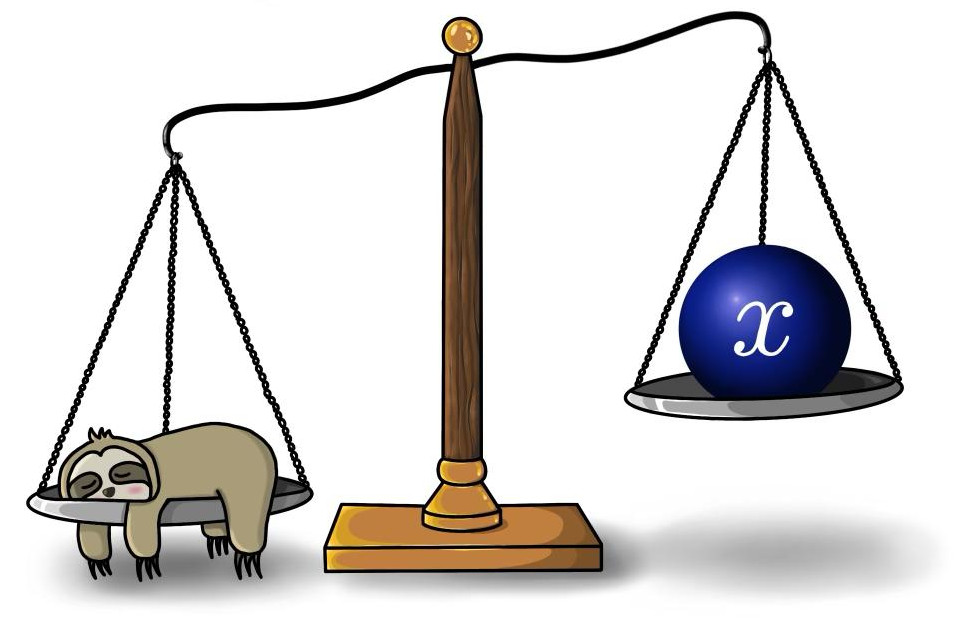
\includegraphics[height=4cm]{images/faultier-balkenwaage.jpg}
\end{center}
\newpage

\vbox{
\begin{example}{}
    \parpic[r]{
        \begin{linearUnequal}
            % Füllung linke Waagschale
            \node[white,marble,inner sep=.12cm] at (-0.85,0.52) {$x$};
            \node[white,marble,inner sep=.12cm] at (-1.15,0.52) {$x$};
            %Füllung rechte Waagschale
            \fill (1.45,0.05) -- (1.05,0.05) -- (1.1,0.4) -- (1.4,0.4) -- cycle;
            \draw[line width=0.75mm] (1.25,0.46) circle[radius=0.06cm];
            \node[white] at (1.25,0.22) {$3$};
            \fill (0.55,0.05) -- (1.05,0.05) -- (1.0,0.45) -- (0.6,0.45) -- cycle;
            \draw[line width=0.75mm] (0.8,0.51) circle[radius=0.06cm];
            \node[white] at (0.8,0.25) {$14$};
        \end{linearUnequal}
    }
    
    Im letzten Beispiel haben wir das mit 3 beschriftete Gewicht auf beiden Seiten der Waage entfernt. Anders ausgedrückt: Wir haben bei der Gleichung $2x+3=17$ auf beiden Seiten den Term 3 subtrahiert.
    
    Hätten wir stattdessen nur auf der linken Seite 3 subtrahiert, dann hätten wir die Gleichung $2x=17$ bekommen -- und die Waage zum Kippen gebracht, weil die linke Seite nun auf einmal leichter als die rechte ist.
\end{example}
}

Wenn wir es also richtig machen machen, dann verändern wir beide Seiten der Gleichung auf die gleiche Weise, zum Beispiel, indem wir auf beiden Seiten $-3$ rechnen. Um alles übersichtlich zu halten, schreiben wir eine neue Gleichung, die wir durch eine Äquivalenzumformung erhalten, nicht neben die alte Gleichung, sondern darunter. Außerdem solltest du darauf achten, dass die Gleichheitszeichen untereinander stehen.

Wenn du darüber hinaus auch noch auf einen Blick sehen möchtest, wie du die Seiten der Gleichung verändert hast, um die untere zu bekommen, dann kannst du diese Rechnung rechts neben der ersten Gleichung noch zusätzlich aufschreiben. Wenn du
\begin{align*}
    \tag{vorher}2x+3&=17\commentLine{-3}\\
    \tag{nachher}2x&=14.
\end{align*}
schreibst, dann kannst du später auf einen Blick sehen, dass du auf beiden Seiten der oberen Gleichung $3$ subtrahieren musst, um die untere Gleichung zu erhalten. Den Strich verwenden wir, damit es wirklich eindeutig ist, dass \enquote{$-3$} nicht mehr zur Gleichung gehört. Er heißt \textbf{Befehlsstrich}.

Wir schauen uns ein weiteres Beispiel an, in dem sich durch das Entfernen von Gegenständen aus den Waagschalen eine neue, äquivalente Gleichung erzeugen lässt.

\begin{example}{}
    \begin{center}
        \begin{linearEquation}
            %Füllung linke Waagschale
            \node[white,marble,inner sep=.12cm] at (-0.85,0.35) {$x$};
            \node[white,marble,inner sep=.12cm] at (-1.15,0.35) {$x$};
            %Füllung rechte Waagschale
            \fill (0.55,0.25) -- (1.05,0.25) -- (1.0,0.65) -- (0.6,0.65) -- cycle;
            \draw[line width=0.75mm] (0.8,0.71) circle[radius=0.06cm];
            \node[white] at (0.8,0.45) {$9$};
            \node[white,marble,inner sep=.12cm] at (1.2,0.35) {$x$};
        \end{linearEquation}
        \bigarrow{
            \node at (0.4,0.2) {$-$};
            \node[white,marble,inner sep=.1cm] at (0.8,0.2) {\scriptsize $x$};
        }
        \begin{linearEquation}
            %Füllung linke Waagschale
            \node[white,marble,inner sep=.12cm] at (-1,0.35) {$x$};
            %Füllung rechte Waagschale
            \fill (0.75,0.25) -- (1.25,0.25) -- (1.2,0.65) -- (0.8,0.65) -- cycle;
            \draw[line width=0.75mm] (1,0.71) circle[radius=0.06cm];
            \node[white] at (1,0.45) {$9$};
        \end{linearEquation}
    \end{center}
    
    Statt Gewichte zu entfernen, kann man auch Kugeln von der Waage entfernen. Die linke Waage stellt beispielsweise die Gleichung $2x=9+x$ dar. Sowohl auf der linken als auch auf der rechten Waagschale liegt eine Kugel. Wir können links und rechts jeweils eine Kugel entfernen. Da die Kugeln gleich schwer waren, bleibt die Waage dabei im Gleichgewicht.
    
    Wir erhalten die Waage auf der rechten Seite (ohne die entfernten Kugeln). Was übrig bleibt, ist links eine einzelne Kugel (also $x$) und rechts das einzelne Gewicht mit der Beschriftung $9$. 
    \begin{align*}
        \tag{vorher}2x&=9+x\commentLine{-x}\\
        \tag{nachher}x&=9.
    \end{align*}
    Wir erhalten durch Subtrahieren von $x$ auf beiden Seiten also die Gleichung $x=9$, die äquivalent zur vorherigen Gleichung $2x=9+x$ ist.
\end{example}

Während wir in den letzten Beispielen vor allem Gewichte bzw. Kugeln entfernt haben, können wir natürlich auch genau das Gegenteil machen: Gewichte und Kugeln hinzufügen. Solange wir auf beiden Seiten das gleiche hinzufügen, bleibt die Waage im Gleichgewicht (wenn sie vorher schon im Gleichgewicht war).

\begin{example}{}
    \begin{center}
        \begin{linearEquation}
        \end{linearEquation}
        \bigarrow{
            \node at (0.2,0.2) {$+$};
            \node[white,marble,inner sep=.1cm] at (0.9,0.2) {\scriptsize $x$};
            \fill (0.75,0.03) -- (0.35,0.03) -- (0.4,0.38) -- (0.7,0.38) -- cycle;
            \draw[line width=0.75mm] (0.55,0.44) circle[radius=0.06cm];
            \node[white] at (0.55,0.2) {$8$};
        }
        \begin{linearEquation}
            %Füllung linke Waagschale
            \fill (-1.45,0.25) -- (-0.95,0.25) -- (-1,0.65) -- (-1.4,0.65) -- cycle;
            \draw[line width=0.75mm] (-1.2,0.71) circle[radius=0.06cm];
            \node[white] at (-1.2,0.45) {$8$};
            \node[white,marble,inner sep=.12cm] at (-0.8,0.35) {$x$};
            %Füllung rechte Waagschale
            \fill (0.55,0.25) -- (1.05,0.25) -- (1.0,0.65) -- (0.6,0.65) -- cycle;
            \draw[line width=0.75mm] (0.8,0.71) circle[radius=0.06cm];
            \node[white] at (0.8,0.45) {$8$};
            \node[white,marble,inner sep=.12cm] at (1.2,0.35) {$x$};
        \end{linearEquation}
    \end{center}
    Eine Balkenwaage, auf die wir nichts gelegt haben, befindet sich natürlich zunächst erst einmal im Gleichgewicht -- so wie die Waage auf dem linken Bild. Sie stellt die Gleichung $0=0$ dar.
    
    Auch die rechte Waage befindet sich im Gleichgewicht. Wir haben einfach auf beiden Seiten das gleiche Gewicht und die gleiche Anzahl an Kugeln hinzugefügt. 
    \begin{align*}
        \tag{vorher}0&=0\commentLine{+8+x}\\
        \tag{nachher}8+x&=8+x
    \end{align*}
    Diese Veränderung bringt die Waage selbstverständlich nicht aus dem Gleichgewicht. Deshalb ist die neue Gleichung $8+x=8+x$ äquivalent zur Gleichung $0=0$. 
    
    Beide Gleichungen sind immer erfüllt (also unabhängig davon, welchen Wert wir für $x$ einsetzen).
    Der Wert von $x$ sollte allerdings sinnvollerweise eine Zahl sein. Die Menge aller uns bekannten Zahlen ist die Menge \Real der reellen Zahlen. Da alle reellen Zahlen die Gleichung lösen, haben die Gleichungen die Lösungsmenge $\Solutions=\Real$.
\end{example}

Wie bereits erwähnt, beschreibt das Hinzufügen von Gewichten und Kugeln zur Waage die Addition von Termen, während das Entfernen von Gegenständen die Subtraktion von Termen darstellt. Insgesamt haben wir durch das Entfernen und Hinzufügen von Kugeln und Gewichten bisher also Folgendes gemacht:
\begin{enumerate}
    \item auf beiden Seiten der Gleichung denselben Term addieren
    \item auf beiden Seiten der Gleichung denselben Term subtrahieren
\end{enumerate}

In jedem Fall haben wir gesehen, dass diese Veränderungen die Lösungsmenge nicht verändern. Wir können also ausgehend von einer vorhandenen Gleichung eine äquivalente Gleichung erzeugen, indem wir auf beiden Seiten denselben Term hinzufügen oder entfernen. Dabei ist es völlig egal, wie kompliziert dieser Term ist. Wichtig ist lediglich, dass wir links und rechts \emph{den gleichen Term} addieren bzw. subtrahieren.

\subsection{Gleichungen auf beiden Seiten multiplizieren}

Bisher haben wir gesehen, dass das beiderseitige Hinzufügen bzw. Entfernen von Termen zu einer Gleichung nichts an der Lösungsmenge ändert, also eine Äquivalenzumformung ist. Im folgenden Beispiel nehmen wir eine etwas subtilere Änderung vor.

\begin{example}{}
    \begin{center}
        \begin{linearEquation}
            %Füllung linke Waagschale
            \fill (-0.95,0.25) -- (-0.55,0.25) -- (-0.6,0.6) -- (-0.9,0.6) -- cycle;
            \draw[line width=0.75mm] (-0.75,0.66) circle[radius=0.06cm];
            \node[white] at (-0.75,0.42) {$4$};
            \node[white,marble,inner sep=.12cm] at (-1.2,0.35) {$x$};
            %Füllung rechte Waagschale
            \fill (0.75,0.25) -- (1.25,0.25) -- (1.2,0.65) -- (0.8,0.65) -- cycle;
            \draw[line width=0.75mm] (1,0.71) circle[radius=0.06cm];
            \node[white] at (1,0.45) {$11$};
        \end{linearEquation}
        \bigarrow{
            \node[circle, inner sep=1mm, fill=white] at (0.6,0.2) {$\cdot 2$};
        }
        \begin{linearEquation}
            %Füllung linke Waagschale
            \fill (-0.95,0.25) -- (-0.55,0.25) -- (-0.6,0.6) -- (-0.9,0.6) -- cycle;
            \draw[line width=0.75mm] (-0.75,0.66) circle[radius=0.06cm];
            \node[white] at (-0.75,0.42) {$8$};
            \node[white,marble,inner sep=.12cm] at (-1.05,0.35) {$x$};
            \node[white,marble,inner sep=.12cm] at (-1.35,0.35) {$x$};
            %Füllung rechte Waagschale
            \fill (0.75,0.25) -- (1.25,0.25) -- (1.2,0.65) -- (0.8,0.65) -- cycle;
            \draw[line width=0.75mm] (1,0.71) circle[radius=0.06cm];
            \node[white] at (1,0.45) {$22$};
        \end{linearEquation}
    \end{center}
    Die linke Balkenwaage stellt die Gleichung $x+4=11$ dar. Das bedeutet natürlich, dass alles, was gerade auf der linken Seite der Waage liegt, genauso viel wiegt wie das, was gerade auf der rechten Seite der Waage liegt.
    
    Legen wir nun einfach jeden Gegenstand auf der linken Seite der Waage noch ein weiteres Mal dazu, so erhalten wir links den Term $2x+8$. Anschaulich wiegt dies doppelt so viel wie vorher, denn wir haben einfach alles, was bereits auf der Wage lag, noch ein zweites Mal auf die Waage gelegt.
    
    Dadurch wäre die linke Seite nun aber erstmal doppelt so schwer wie die rechte. Um das auszugleichen, müssen wir auch das Gewicht der rechten Seite verdoppeln, das Gewicht mit der 11 also noch ein weiteres Mal auf die Waage legen. Dadurch verdoppelt sich das Gesamtgewicht auf der rechten Seite auf 22. 
    \begin{align*}
        x+4&=11\commentLine{\cdot 2}\\
        2x+8&=22
    \end{align*}
    Nun, da wir beide Seiten verdoppelt haben, befindet sich die Waage wieder im Gleichgewicht. Daraus, dass die Waage sich nach dem Verdoppeln im Gleichgewicht befindet, kannst du umgekehrt natürlich auch schließen, dass sie vorher schon im Gleichgewicht gewesen sein musste.
\end{example}
Im Beispiel haben wir, statt auf beiden Seiten dieselben Gegenstände zu entfernen oder hinzuzufügen, beide Seiten einzeln betrachtet und jeweils verdoppelt, also beide Seiten mit 2 multipliziert. Genauso wäre es auch möglich gewesen, alles zu verfünffachen oder mit (fast) jeder beliebigen anderen Zahl zu multiplizieren. Bei der Multiplikation mit 5 wären zum Beispiel beide Seiten danach fünfmal so schwer wie vorher, was die Waage auch nicht aus dem Gleichgewicht bringt.

Letztlich haben wir hier jede Seite der Gleichung mit derselben Zahl multipliziert. Ob das nun 2, 5 oder eine andere Zahl ist, spielt keine wirkliche Rolle. Die Werte auf der linken und rechten Seite verändern sich auf diese Weise gleichmäßig und die Gleichung bleibt gültig.

Beim Multiplizieren ist jedoch Vorsicht geboten, weil sich Gleichungen durch unvorsichtiges Multiplizieren schnell zerstören lassen, wie das nächste Beispiel zeigt.

\begin{example}{}
    \begin{center}
        \begin{linearUnequal}
            %Füllung linke Waagschale
            \fill (-0.75,0.43) -- (-1.25,0.43) -- (-1.2,0.83) -- (-0.8,0.83) -- cycle;
            \draw[line width=0.75mm] (-1,0.89) circle[radius=0.06cm];
            \node[white] at (-1,0.63) {$14$};
            %Füllung rechte Waagschale
            \fill (0.75,0.07) -- (1.25,0.07) -- (1.2,0.47) -- (0.8,0.47) -- cycle;
            \draw[line width=0.75mm] (1,0.53) circle[radius=0.06cm];
            \node[white] at (1,0.27) {$16$};
        \end{linearUnequal}
        \bigarrow{
            \node[circle, inner sep=1mm, fill=white] at (0.6,0.2) {$\cdot 0$};
        }
        \begin{linearEquation}
        \end{linearEquation}
    \end{center}
    Wir beginnen diesmal mit einer Waage, die sich offensichtlich nicht im Gleichgewicht befindet: Sie stellt die Gleichung $14=16$ dar, die natürlich nicht gilt, denn die Zahlen sind ja verschieden.
    
    Auch wenn wir die Gleichung mit einer Zahl wie 3 oder 7 multiplizieren, bleibt die rechte Seite schwerer als die linke. Das ist auch gut so, denn wenn die Waage auf einmal im Gleichgewicht wäre, dann hätte die Gleichung auf einmal eine Lösung (und wäre damit nicht äquivalent zur Gleichung $14=16$, die keine Lösung hat). 
    
    Stattdessen multiplizieren wir die Gleichung nun aber mit 0, entfernen also effektiv alle Gegenstände von der Waage.
    Das Ergebnis ist eine leere Waage, die die Gleichung $0=0$ repräsentiert und sich wieder im Gleichgewicht befindet. Weil die Waage vorher aber nicht im Gleichgewicht war, zeigt dies, dass wir \emph{keine Äquivalenzumformung} vorgenommen haben: Die Gleichungen $14=16$ und $0=0$ verhalten sich vollkommen unterschiedlich, denn eine der beiden Aussagen ist offenbar immer wahr, die andere immer falsch.
\end{example}

Im Beispiel haben wir gesehen, dass es unklug ist, eine Gleichung mit 0 zu multiplizieren. Das kann man zwar machen, aber die dann entstehende Gleichung ist nicht äquivalent zur ursprünglichen. Stattdessen erhält man die immer erfüllte Gleichung $0=0$, die ziemlich langweilig ist. Insbesondere sagt sie nichts über das gesuchte $x$ in der ursprünglichen Gleichung aus.

Das Multiplizieren beider Seiten mit einer Zahl ist normalerweise eine Äquivalenzumformung, wie das vorletzte Beispiel gezeigt hat. Allerdings dürfen wir eine Gleichung \emph{niemals mit 0 multiplizieren}, weil wir dann immer die Gleichung $0=0$ erhalten, mit der wir nichts anfangen können.

Wenn wir den Wert der Unbekannten $x$ suchen, die in einer Gleichung vorkommt, dann können wir erstmal nicht sagen, ob sie vielleicht den Wert $0$ hat. Da wir eine Gleichung aber nicht mit $0$ multiplizieren dürfen, ist es auch nicht sinnvoll, eine Gleichung mit $x$ zu multiplizieren. Außerdem dürfen wir die Gleichung auch nicht durch $x$ teilen, denn es ist nicht möglich, durch $0$ zu teilen.

Bevor wir zusammenfassen, welche Äquivalenzumformungen wir bisher gesehen haben, betrachten wir noch ein weiteres Beispiel. Es wird darauf hinauslaufen, dass wir beide Seiten einer Gleichung durch dieselbe Zahl dividieren.

\begin{example}{}
    \begin{center}
        \begin{linearEquation}
            %Füllung linke Waagschale
            \node[white,marble,inner sep=.12cm] at (-1.3,0.35) {$x$};
            \node[white,marble,inner sep=.12cm] at (-1,0.35) {$x$};
            \node[white,marble,inner sep=.12cm] at (-0.7,0.35) {$x$};
            %Füllung rechte Waagschale
            \fill (0.75,0.25) -- (1.25,0.25) -- (1.2,0.65) -- (0.8,0.65) -- cycle;
            \draw[line width=0.75mm] (1,0.71) circle[radius=0.06cm];
            \node[white] at (1,0.45) {$18$};
        \end{linearEquation}
        \bigarrow{
            \node[circle, inner sep=1mm, fill=white] at (0.6,0.2) {$\div 3$};
        }
        \begin{linearEquation}
            %Füllung linke Waagschale
            \node[white,marble,inner sep=.12cm] at (-1,0.35) {$x$};
            %Füllung rechte Waagschale
            \fill (0.75,0.25) -- (1.25,0.25) -- (1.2,0.65) -- (0.8,0.65) -- cycle;
            \draw[line width=0.75mm] (1,0.71) circle[radius=0.06cm];
            \node[white] at (1,0.45) {$6$};
        \end{linearEquation}
    \end{center}
    Links sehen wir, wie die Gleichung $3x=18$ auf einer Balkenwaage dargestellt ist. Wir können sofort sagen, dass das Gesamtgewicht auf der linken Seite dreimal so groß ist wie das einer einzelnen Kugel. Wir können nun beginnen und zwei der drei Kugeln entfernen, wodurch auf der linken Seite dann nur noch eine Kugel (also $x$) übrig bleibt. Natürlich verändert das aber das Gewicht auf der linken Seite und wir müssen irgendetwas mit der rechten Seite machen, damit die Waage nicht aus dem Gleichgewicht kommt.
    
    Wie genau hat sich das Gewicht links also verändert? Im Wesentlichen ist das ganz einfach zu beantworten: Wir hatten vorher drei Kugeln, jetzt haben wir nur noch eine. Das Gewicht ist also nur noch ein Drittel vom ursprünglichen Gewicht. Dadurch ist auch klar, was auf der rechten Seite zu tun ist: Wir müssen das Gewicht auf der rechten Seite durch 3 teilen. Dort erhalten wir also $18:3=6$.
    
    Schließlich führt das zur Waage auf der rechten Seite, die die Gleichung $x=6$ darstellt. Mittlerweile liegt auf beiden Seiten nur noch ein Drittel des ursprünglichen Gewichts, aber da wir beide Seiten durch 3 geteilt haben, ist die Waage immer noch im Gleichgewicht.
    
    In diesem Beispiel haben wir also beide Seiten mit $\frac{1}{3}$ multipliziert oder (weil das genau dasselbe ist) beide Seiten durch 3 geteilt.
    \begin{align*}
        3x&=18\commentLine{\div 3}\\
        x&=6.
    \end{align*}
\end{example}

Wir haben jetzt insgesamt vier verschiedene Äquivalenzumformungen gesehen:
\begin{enumerate}
    \item die Addition eines Terms auf beiden Seiten
    \item die Subtraktion eines Terms auf beiden Seiten
    \item die Multiplikation beider Seiten mit einem Term, \textbf{der nicht den Wert 0 hat}
    \item die Division beider Seiten durch einen Term, \textbf{der nicht den Wert 0 hat}
\end{enumerate}

Damit haben wir die wichtigsten Werkzeuge beisammen, um Gleichungen so umzuformen, dass wir herausfinden können, für welche Werte für $x$ sie erfüllt sind. Der folgende Satz drückt noch einmal aus, dass die Veränderungen, die wir gerade zusammengefasst haben, Äquivalenzumformungen sind. All das, was wir uns gerade mithilfe von Balkenwaagen überlegt haben, lässt sich theoretisch auch mathematisch beweisen.

\begin{theorem}[th:equivalent-transformations]{Äquivalenzumformungen}
    Die Lösungsmenge einer Gleichung bleibt unverändert, wenn man
    \begin{itemize}
        \item zu jeder Seite eine Zahl $a\in\mathbb{R}$ addiert.
        \item jede Seite mit einer Zahl $a\neq 0$ multipliziert.
    \end{itemize}
\end{theorem}

\vfill
\begin{center}    
    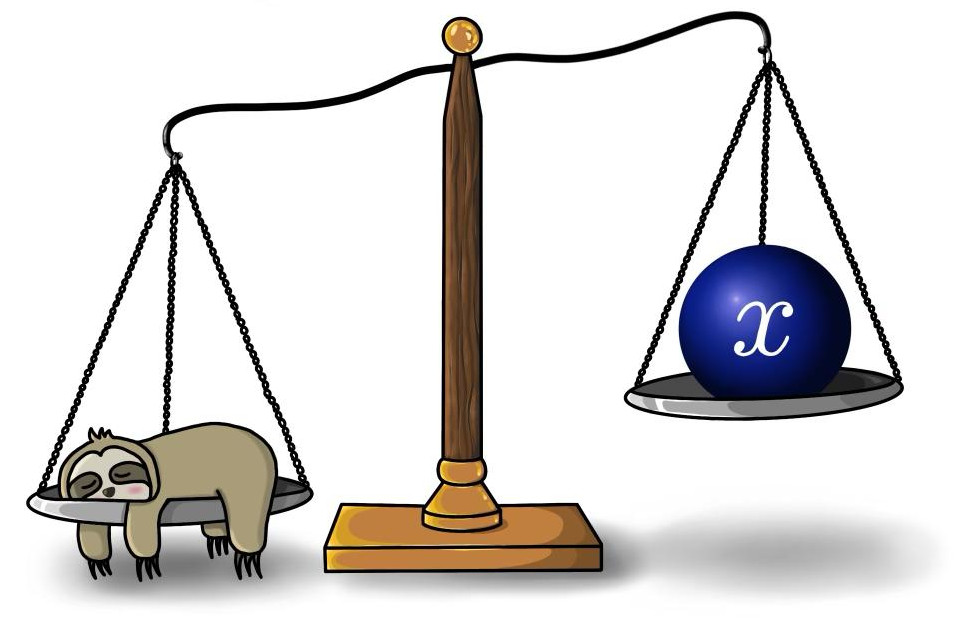
\includegraphics[height=7cm]{images/faultier-balkenwaage.jpg}
\end{center}
\newpage

\begin{advanced}{Kürzungsregel}
    Dass sich die Lösungsmenge einer Gleichung bei den Äquivalenzumformungen, die im obigen Satz beschrieben sind, nicht ändert, haben wir uns auf den letzten Seiten anschaulich mithilfe von Balkenwaagen überlegt. Formal lässt sich die Korrektheit von Äquivalenzumformungen mit der Kürzungsregel für die Addition und Multiplikation beweisen.
    
    \begin{theorem}{Kürzungsregel}
        Es seien $a,b\in\Real$. Dann gilt: 
        \begin{enumerate}
            \item Für alle $c\in\Real$ ist $a+c=b+c$ genau dann, wenn $a=b$.
            \item Für alle $c\in\Real$ mit $c\neq 0$ gilt $ac=bc$ genau dann, wenn $a=b$.
        \end{enumerate}
    \end{theorem}
    
    Die Kürzungsregel beruht darauf, dass die Addition und die Multiplikation auf den reellen Zahlen eine \emph{Gruppenstruktur} erzeugen. Eine detailliertere Erläuterung, was eine Gruppe ist, kannst du ebenso wie den Beweis der Kürzungsregel auf Seite \pageref{} finden. 
\end{advanced}

Neben den Grundrechenarten, die Beispiele für Äquivalenzumformungen sind, kennen wir bereits andere Rechenarten, die \emph{keine} Äquivalenzumformungen sind. Eine davon ist das Wurzelziehen.

\begin{example}{}
    In Beispiel \ref{ex:sqrt-umformung} ist uns bereits einmal die Gleichung $x^2=4$ begegnet. Wenn wir auf beiden Seiten die Wurzel ziehen, erhalten wir links $\sqrt{x^2}$, also $x$. Rechts bekommen wir $\sqrt{4}$, also $2$. Die neue Gleichung nach dem Wurzelziehen ist also $x=2$. Du weißt aber bereits aus Beispiel \ref{ex:sqrt-umformung}, dass diese beiden Gleichungen nicht äquivalent sind, weil $x^2=4$ die Lösung $-2$ hat, die es bei der Gleichung $x=2$ nicht gibt.
\end{example}

Achte, wenn du Gleichungen umformst, also immer darauf, dass die Umformung, die du vornimmst, eine Äquivalenzumformung ist. Falls du das nicht tust, entstehen Schwierigkeiten, die du zusätzlich beachten musst.

\begin{nutshell}{Äquivalenzumformungen}
    Für jede Gleichung kann es Werte geben, die sich für die Unbekannte $x$ einsetzen lassen, sodass die Gleichung erfüllt ist. Allerdings \emph{muss} es diese Werte nicht geben. Beispielsweise hat die Gleichung $x=x+2$ keine Lösungen. Die Menge aller Werte, die für $x$ eingesetzt werden können, sodass eine bestimmte Gleichung erfüllt ist, heißt die \textbf{Lösungsmenge} \Solutions \emph{dieser} Gleichung.
    
    Manche Gleichungen haben dieselbe Lösungsmenge, obwohl sie eigentlich unterschiedlich sind. Die Gleichungen $x+15=20$ und $x=5$ haben beispielsweise beide die Lösungsmenge $\Solutions=\{5\}$. Zwei Gleichungen, die die gleiche Lösungsmenge haben, heißen \textbf{äquivalent}. Es gibt bestimmte Umformungen, die wir an einer Gleichung durchführen können, um immer eine äquivalente Gleichung zu bekommen:
    \begin{itemize}
        \item auf beiden Seiten denselben Wert addieren
        \item auf beiden Seiten denselben Wert subtrahieren
        \item beide Seiten mit demselben Wert multiplizieren (aber nicht mit 0)
        \item beide Seiten durch denselben Wert dividieren (aber nicht durch 0)
    \end{itemize}
    Solche Umformungen heißen \textbf{Äquivalenzumformungen}. Nicht jede Rechenoperation ist eine Äquivalenzumformung. Das Wurzelziehen ist beispielsweise keine Äquivalenzumformung, weil dabei Lösungen verloren gehen.
\end{nutshell}

\end{document}